\subsection{Path loss models}

In terms of calculating the PL, different propagation models can be applied, to calculate the power received, given different conditions. One of the more extensive models is Ground Wave Path Loss (GWPL) model. The GWPL model takes the three most dominant factors into account when calculating the PL \cite{Chong,Bullington}, the direct wave the reflected wave and the surface wave.  


\begin{equation}
P_r=P_0 \cdot \Big|\underbrace{1}_{\begin{subarray}{c}Direct\\wave\end{subarray}}+\underbrace{R\text{e}^{j\Delta}}_{\begin{subarray}{c}Reflected\\wave\end{subarray}}+\underbrace{(1-R)A\text{e}^{j\Delta}}_{\begin{subarray}{c}Surface\\wave\end{subarray}}\Big|^2 
\label{ground_wave}
\end{equation}
where
\begin{equation}
P_0 = \frac{P_t G_t G_r}{L} \left(\frac{\lambda}{4 \pi d}\right)^2 
\label{ground_wave_P0}
\end{equation}

$P_{r}$ and $P_{t}$ are the power received and transmitted respectively, $G_t$ and $G_r$ are the gains in the transmitting and receiving antenna respectively, $L$ is the system loss, $\lambda$ is the wavelength of the transmitted signal, $d$ is the distance between the transmitting and receiving antenna, $\Delta$ is the phase difference between the direct and reflected wave, $R$ is the complex reflection coefficient and $A$ is the surface wave attenuation factor \cite{Chong,Bullington}. 

%$\Delta$ $\approx$ $\frac{4\pi h_{r} h_{t}}{\lambda d}$

The complex reflection coefficient is dependent on the incidence angle and the surface materiel.
\begin{equation}
R = \frac{\sin(\theta)-z}{\sin(\theta)-z}
\label{reflection_coefficient}
\end{equation}

where $\theta$ is the incidence angle and $z$ is different for vertical or horizontal polarization, and respectively given as.

\begin{align}
z &= \frac{\sqrt{\epsilon_{0}-\cos^{2}\theta}}{\epsilon_{0}} \\
z &= \sqrt{\epsilon_{0}-\cos^{2}\theta}
\end{align}

where $\epsilon_{0}$ is the Complex relative permittivity for the surface and can be found using the methods described in \cite{Kim}.\\
The surface wave attenuation factor can approximated as \eqref{attenuation_factor_A}\cite{Chong, Bullington}. 


\begin{equation}
A \approx \frac{-1}{1+j\frac{2\pi d}{\lambda}(\sin(\theta)+z)^{2}}
\label{attenuation_factor_A}
\end{equation}


As the GWPL model is quite complex different approximations of it has been made that makes it possible to calculate the PL without making measurements of the environment. The most simple model is the Friss free space path loss (FSPL) model \eqref{simple_friss} which calculates the power received, given only free space loss \cite{Chong}. This means that the reflected wave and surface wave can be set to 0 in \eqref{ground_wave}. 

\begin{equation}
P_r = \frac{P_t G_t G_r}{L} \left(\frac{\lambda}{4 \pi d}\right)^2
\label{simple_friss}
\end{equation}

This model \eqref{simple_friss} is not the the complete FSPL, as it assumes no losses due to polarization mismatch, pointing error, and matching between the system and antennas \cite{full_friss}. \\



As the FSPL only accounts for the direct wave between the receiver and the transmitter. A model that also accounts for the single point reflected wave is the two-ray-ground-reflection path loss model (TRPL) \cite{two_ray}. 

\begin{equation}
P_r(d) = \frac{P_t G_t G_r }{L}\left(\frac{h_t h_r}{d^2}\right)^2
\label{two_ray_model}
\end{equation}

where $h_t$, $h_r$ are the heights of the transmitting and receiving antenna respectively. \\
From the complete ground wave model given in \eqref{ground_wave}, the TRLP can be simplified to \eqref{two_ray_model}, when $\frac{\Delta}{2}$ $<$ $\pi$/$10$ $\Rightarrow$ $\sin$ $\frac{\Delta}{2}$ $\approx$ $\frac{\Delta}{2}$. This approximation holds when \eqref{two_ray_cond} is true and thus the simplified TRPL \eqref{two_ray_model} can be applied. If \eqref{two_ray_cond} is false FSPL \eqref{simple_friss} can be applied.
  
\begin{equation}
d > \frac{4\pi \cdot h_t h_r }{\lambda}
\label{two_ray_cond}
\end{equation}
 

The condition \eqref{two_ray_cond}, is because the TRPL model considers two waves, a direct and a reflected wave, which interferes in an alternating constructive or destructive manner. If the condition is true use FSPL, while if false use TRPL.   %The cross over distance $d_c$ can be found using \eqref{two_ray_cross_dis} \cite{two_ray}. 
\\

%\begin{equation}
%P_r(d) = \frac{P_t G_t G_r }{L}\left(\frac{h_t h_r}{d^2}\right)^2
%\label{two_ray_model}
%\end{equation}

%where $h_t$, $h_r$ are the heights of the transmitting and receiving antenna respectively. \\
%As the TRPL model considers two waves, a direct and a reflected wave, this model predicts interferences, which are caused by the constructive and destructive combination of the two waves. The interference is dominant if \eqref{two_ray_cond} is true\cite{two_ray}.


%this gives the following condition:


%a condition is introduced given as:

%\begin{equation}
%d < d_{c}
%\label{two_ray_cond}
%\end{equation}

%where %$d_{c}$ is called the cross over distance and is given as:

%\begin{equation}
%d_{c} = \frac{4\pi \cdot h^2_t h^2_r }{\lambda}
%\label{two_ray_cross_dis}
%\end{equation}  

However when placing the antennas at ground level, the TRLP predicts that the power received is zero, which is not the case.
The reason is that another wave becomes a factor. This wave is called the surface wave \cite{Chong}. The surface wave assumes a minimum effective height of the antennas as can be seen in \eqref{surface_wave}. 

\begin{equation}
P_r=\frac{P_t G_t G_r }{L}\left(\frac{h_0}{d}\right)^4
\label{surface_wave}
\end{equation}

where $h_0$ is the minimum effective height of the antennas.  This equation assume that the phase difference between reflected and direct wave is $\approx 0$ and the reflection coefficient $\approx -1$. The condition in terms of when to use the surface wave is depending on the height of the antennas \cite{Chong}.
\begin{equation}
h_{r,t} < \lambda
\label{cond_surface}
\end{equation}
When \eqref{cond_surface} is true the FSPL and TRPL respectively under and overestimate the PL.
While when both of the antennas are elevated at least one $\lambda$ above ground, or 5-10 $\lambda$ above water \cite{Chong}, the surface wave can be neglected. 

\begin{figure}[!htbp]
% This file was created by matlab2tikz.
%
%The latest updates can be retrieved from
%  http://www.mathworks.com/matlabcentral/fileexchange/22022-matlab2tikz-matlab2tikz
%where you can also make suggestions and rate matlab2tikz.
%
\definecolor{mycolor1}{rgb}{0.00000,0.44700,0.74100}%
\definecolor{mycolor2}{rgb}{0.85000,0.32500,0.09800}%
\definecolor{mycolor3}{rgb}{0.92900,0.69400,0.12500}%
\definecolor{mycolor4}{rgb}{0.49400,0.18400,0.55600}%
%
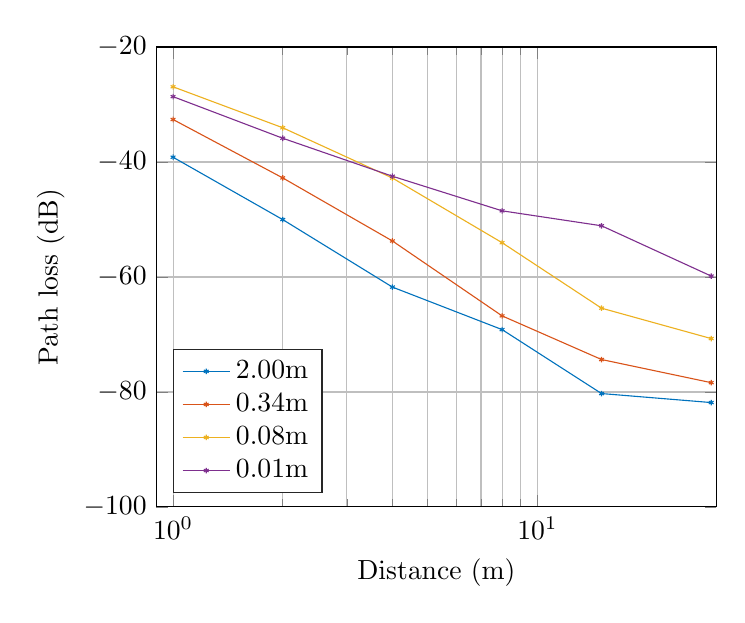
\begin{tikzpicture}

\begin{axis}[%
width=2.8in,
height=2.3in,
at={(2.08in,0.858in)},
scale only axis,
xmode=log,
xmin=0.9,
xmax=31,
xlabel=Distance (m),
xminorticks=true,
xmajorgrids,
xminorgrids,
ymin=-100,
ymax=-20,
ylabel=Path loss (dB),
ymajorgrids,
legend pos = south west,
axis background/.style={fill=white},
legend style={legend cell align=left,align=left,draw=white!15!black}
]
\addplot [color=mycolor1,solid,mark size=1.0pt,mark=asterisk,mark options={solid}]
  table[row sep=crcr]{%
1	-39.176832441447\\
2	-50.0236813268286\\
4	-61.7627349006033\\
8	-69.1568155321866\\
15	-80.2784721484843\\
30	-81.8463231335614\\
};
\addlegendentry{2.00m};

\addplot [color=mycolor2,solid,mark size=1.0pt,mark=asterisk,mark options={solid}]
  table[row sep=crcr]{%
1	-32.6162301822822\\
2	-42.7733202106742\\
4	-53.7406598744587\\
8	-66.7692891298477\\
15	-74.3619892107941\\
30	-78.384604174472\\
};
\addlegendentry{0.34m};

\addplot [color=mycolor3,solid,mark size=1.0pt,mark=asterisk,mark options={solid}]
  table[row sep=crcr]{%
1	-26.9292301822822\\
2	-34.0517673842044\\
4	-42.7927848744587\\
8	-54.0404141298477\\
15	-65.4297392107941\\
30	-70.718229174472\\
};
\addlegendentry{0.08m};

\addplot [color=mycolor4,solid,mark size=1.0pt,mark=asterisk,mark options={solid}]
  table[row sep=crcr]{%
1	-28.6391813268286\\
2	-35.8754849006033\\
4	-42.4804405321866\\
8	-48.4989721484843\\
15	-51.0989481335614\\
30	-59.847479174472\\
};
\addlegendentry{0.01m};

\end{axis}
\end{tikzpicture}%
\end{figure}

